\documentclass[a4paper,11pt]{article}
\usepackage{amsmath,amsthm,amsfonts,amssymb,amscd,amstext,vmargin,graphics,graphicx,tabularx,multicol} \usepackage[french]{babel}
\usepackage[utf8]{inputenc}  
\usepackage[T1]{fontenc} 
\usepackage[T1]{fontenc}
\usepackage{amsmath,amssymb}
\usepackage{pstricks-add,tikz,tkz-tab,variations}
\usepackage[autolanguage,np]{numprint} 
\usepackage{color}
\usepackage{ulem}

\setmarginsrb{1.5cm}{0.5cm}{1cm}{0.5cm}{0cm}{0cm}{0cm}{0cm} %Gauche, haut, droite, haut
\newcounter{numexo}
\newcommand{\exo}[1]{\stepcounter{numexo}\noindent{\bf Exercice~\thenumexo} : \marginpar{\hfill /#1}}
\reversemarginpar


\newcounter{enumtabi}
\newcounter{enumtaba}
\newcommand{\q}{\stepcounter{enumtabi} \theenumtabi.  }
\newcommand{\qa}{\stepcounter{enumtaba} (\alph{enumtaba}) }
\newcommand{\initq}{\setcounter{enumtabi}{0}}
\newcommand{\initqa}{\setcounter{enumtaba}{0}}

\newcommand{\be}{\begin{enumerate}}
\newcommand{\ee}{\end{enumerate}}
\newcommand{\bi}{\begin{itemize}}
\newcommand{\ei}{\end{itemize}}
\newcommand{\bp}{\begin{pspicture*}}
\newcommand{\ep}{\end{pspicture*}}
\newcommand{\bt}{\begin{tabular}}
\newcommand{\et}{\end{tabular}}
\renewcommand{\tabularxcolumn}[1]{>{\centering}m{#1}} %(colonne m{} centrée, au lieu de p par défault) 
\newcommand{\tnl}{\tabularnewline}

\newcommand{\trait}{\noindent \rule{\linewidth}{0.2mm}}
\newcommand{\hs}[1]{\hspace{#1}}
\newcommand{\vs}[1]{\vspace{#1}}

\newcommand{\N}{\mathbb{N}}
\newcommand{\Z}{\mathbb{Z}}
\newcommand{\R}{\mathbb{R}}
\newcommand{\C}{\mathbb{C}}
\newcommand{\Dcal}{\mathcal{D}}
\newcommand{\Ccal}{\mathcal{C}}
\newcommand{\mc}{\mathcal}

\newcommand{\vect}[1]{\overrightarrow{#1}}
\newcommand{\ds}{\displaystyle}
\newcommand{\eq}{\quad \Leftrightarrow \quad}
\newcommand{\vecti}{\vec{\imath}}
\newcommand{\vectj}{\vec{\jmath}}
\newcommand{\Oij}{(O;\vec{\imath}, \vec{\jmath})}
\newcommand{\OIJ}{(O;I,J)}

\newcommand{\bmul}[1]{\begin{multicols}{#1}}
\newcommand{\emul}{\end{multicols}}


\newcommand{\reponse}[1][1]{%
\multido{}{#1}{\makebox[\linewidth]{\rule[0pt]{0pt}{20pt}\dotfill}
}}

\newcommand{\titre}[5] 
% #1: titre #2: haut gauche #3: bas gauche #4: haut droite #5: bas droite
{
\noindent #2 \hfill #4 \\
#3 \hfill #5

\vspace{-1.6cm}

\begin{center}\rule{6cm}{0.5mm}\end{center}
\vspace{0.2cm}
\begin{center}{\large{\textbf{#1}}}\end{center}
\begin{center}\rule{6cm}{0.5mm}\end{center}
}



\begin{document}
\pagestyle{empty}
\titre{Interrogation : Géométrie dans l'espace}{Nom}{Prénom}{Date}{Classe}
\vspace*{0.5cm}


\exo{5}On considère la pyramide ABCD de hauteur [AD] telle que AD = 5 cm et de base ABC telle que AB = 4,8 cm ; BC = 3,6 cm ; CA = 6 cm. \\
(La figure n'est pas aux dimensions.)

\bmul{2}

\noindent \initq \q Démontrer que le triangle ABC est rectangle en B.\\
\q Calculer le volume de cette pyramide au centième près.\\
\q On désire fabriquer de telles pyramides en plâtre. Combien peut-on en obtenir avec 1 $dm^{3}$ de plâtre ?\\
\vspace*{0.5cm}

\columnbreak

\begin{center}
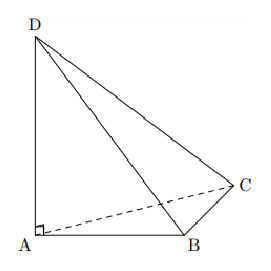
\includegraphics[scale=1]{volpyramide.eps} 
\end{center}

\emul


\noindent \reponse[25]\\

\newpage

\vspace*{0.4cm}

\exo{5} Le cône de révolution ci-dessous de sommet S a une hauteur [SO] de 9 cm et un rayon de base [OA] de 5 cm.\\
\initq 

\q Calculer le volume $V_{1}$ de ce cône au  $cm^{3}$ près.\\

\q Soit M le point du segment [SO] tel que SM = 3 cm. On coupe le cône par un plan parallèle à la base passant par M.\\

\qa Quelle est la nature du solide que l'on obtient alors ? Est-ce une réduction ou un agrandissement du cône de révolution initial ?  En déduire le coefficient de réduction ou d'agrandissement. Justifier votre réponse.\\


\qa Calculer le volume $V_{2}$  du nouveau solide de sommet S ainsi obtenu au $cm^{3}$ près, en utilisant la méthode de votre choix\\


\bmul{2}

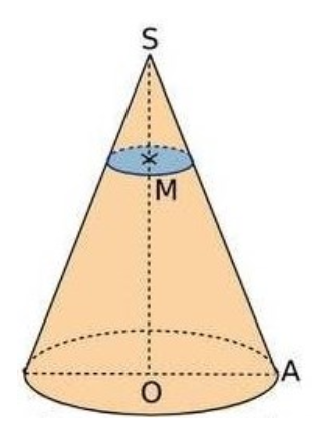
\includegraphics[scale=0.6]{coneinterro.eps} 


\columnbreak

\noindent \reponse[7]


\emul


\noindent \reponse[20]






\end{document}
